% preamble includes document settings
\documentclass[12pt,letterpaper]{article}

% use Unicode characters - try changing the option if you run into troubles with special characters (e.g. umlauts)
\usepackage[utf8]{inputenc}

% clean citations
% see https://tex.stackexchange.com/questions/284982/cse-citation-style#285252
\usepackage[round,sort&compress]{natbib}
\setcitestyle{aysep={},citesep={,}}

% hyperref makes references clicky. use \url{www.example.com} or \href{www.example.com}{description} to add a clicky url
\usepackage{nameref,hyperref}

% line numbers
\usepackage[right]{lineno}

% improves typesetting in LaTeX
\usepackage{microtype}
\DisableLigatures[f]{encoding = *, family = * }

% text layout - change as needed
\raggedright
\setlength{\parindent}{0.5cm}
\textwidth 5.25in 
\textheight 8.75in

% Remove % for double line spacing
\usepackage{setspace} 
\doublespacing

% use adjustwidth environment to exceed text width (see examples in text)
\usepackage{changepage}

% adjust caption style
\usepackage[aboveskip=1pt,labelfont=bf,labelsep=period,singlelinecheck=off]{caption}

% remove brackets from references
\makeatletter
\renewcommand{\@biblabel}[1]{\quad#1.}
\makeatother

% headrule, footrule and page numbers
\usepackage{lastpage,fancyhdr,graphicx}
\usepackage{epstopdf}

% use \textcolor{color}{text} for colored text (e.g. highlight to-do areas)
\usepackage{color}

% define custom colors (this one is for figure captions)
\definecolor{Gray}{gray}{.25}

% this is required to include graphics
\usepackage{graphicx}

% use if you want to put caption to the side of the figure - see example in text
\usepackage{sidecap}

% use for have text wrap around figures
\usepackage{wrapfig}
\usepackage[pscoord]{eso-pic}
\usepackage[fulladjust]{marginnote}
\reversemarginpar

\providecommand{\keywords}[1]{\textbf{\textit{Keywords---}} #1}

% to support doublespacing
\usepackage{setspace}

% set doublespacing for captions
\DeclareCaptionJustification{double}{\doublespacing}
\captionsetup{justification=double}



% document begins here
\begin{document}

\begin{flushleft}

{\Large
 \textbf\newline{Toward Reliable Biodiversity Dataset References}
 }
 \newline
% authors go here:
Michael J. Elliott\textsuperscript{1}\textsuperscript{†},
Jorrit H. Poelen\textsuperscript{2}\textsuperscript{†}\textsuperscript{*},
José A.B. Fortes\textsuperscript{1}
\bigskip
\\
\bf{\textsuperscript{1}} Advanced Computing and Information Systems Laboratory (ACIS)\\Department of Electrical and Computer Engineering, University of Florida, Gainesville, FL\\339 Larson Hall, PO Box 116200, Gainesville, Florida 32611-6200, USA
\\
\bf{\textsuperscript{2}} Ronin Institute for Independent Scholarship, Montclair, NJ, USA
\\
\bf{\textsuperscript{†}} These authors contributed equally to this work
\\
\bf{\textsuperscript{*}} Corresponding author
\bigskip


\end{flushleft}



\clearpage
\newpage

% title goes here:
\begin{flushleft}
{\Large
\textbf\newline{Toward Reliable Biodiversity Dataset References}
}
\newline
\end{flushleft}

% now start line numbers
\linenumbers

%\clearpage makes sure that all above content is printed at this point and does not invade into the upcoming content
%\clearpage

\begin{abstract}
% Points

% -- Qualify link rot and content drift
% -- Observatory can monitor link rot, content drift
% -- Proposed content hash citation
\noindent
No systematic approach has yet been adopted to reliably reference and provide access to digital biodiversity datasets. Based on accumulated evidence, we argue that location-based identifiers such as URLs are not sufficient to ensure long-term data access. We introduce a method that uses dedicated data observatories to evaluate long-term URL reliability.

From March though October of 2019, we took periodic inventories of the data served by major biodiversity aggregators, including GBIF, iDigBio, DataONE, and BHL. Over the period of observation, we found that, for each network, 5% to 43% of registered URLs were intermittently or consistently unresponsive, 0% to 63% produced unstable content, and 13% to 76% became either unresponsive or unstable.

We propose the use of cryptographic hashing to generate content-based identifiers that can reliably reference datasets. We show that content-based identifiers facilitate decentralized archival and reliable distribution of biodiversity datasets to enable long-term accessibility of the referenced datasets.
\end{abstract}

\keywords{Biodiversity, Ecological Informatics, Information Systems, Information Retrieval}



\section*{Introduction}
Over the course of hundreds of years, naturalists and biologists have systematically collected physical evidence from an ever-changing natural world. Through well-established protocols and institutional support, many of these natural history collections have withstood the ravages of time \citep{Hortal_2015,Davis_1996}. Records that describe these carefully collected specimens are now made available digitally through online search indices, registries, and data archives \citep{Page_2015}. The increased availability of digital natural history records helps realize Charles Elton's vision of ``[linking] up into some complete scheme the colossal store of facts about natural history which has accumulated up to date in this rather haphazard manner'' \citep{Elton_1927}. So far, various initiatives have succeeded in providing comprehensive aggregate views from previously scattered natural history record siloes \citepalias{Rinaldo_2009,Michener_2011,Edwards_2000,matsunaga2013integrated,gbif_org_2019}. However, we show that these aggregate views are subject to change as their underlying digital source data changes or becomes inaccessible. Although efforts have been made to track changes in dataset networks with versioning, last-modified dates \citep{Wieczorek_2012,Robertson_2014}, and periodic archiving \citep{Costello_2013}, , no systematic approach has been adopted to keep our digital natural history record accessible. Despite centuries of expertise in preserving our physical natural history records, biologists currently struggle to maintain a growing body of digital data that can change or disappear with the push of a button.

Our scholarly record consists of an intricate web of associations between scientific studies and the datasets on which they are based. These associations are made explicit through citations that can be used to reconstruct a study's context and provide the chain of evidence that supports its claims \citep{Garfield_1964}. In the pre-internet era, the lookup of cited references required access to one or more of the many academic libraries in the world. With the rise of internet-accessible scientific publications, authors and readers access these references by using a networked device to download content from publication websites. This means that researchers are increasingly citing online works to support their claims. Because the citation format of online works typically documents only when (e.g., 2019-10-01) and where (e.g., https://doi.org/10.123/456) the referenced work was accessed by the author \citepalias{gbif_2019,idigbio_2016,dataone_2012}, the reader expects the web-accessed resource to remain accessible and unaltered via this single web location. Readers may attempt to find a version of the works referenced by searching online data networks for the matching author and title, but there is no guarantee that information found this way will be exactly the same as what was originally referenced. Any reference that does not allow readers to find the referenced work fails to satisfy the FAIR principle of findability: ``F1. (meta)data are assigned a globally unique and eternally persistent identifier'' \citep{Wilkinson_2016}. Our study supports Klein’s and Vision’s findings that networked, location-based access to digital objects is an unreliable mechanism for providing continued access to the unaltered original work \citep{Vision_2010,Klein_2014}. Unless we change the way we preserve and cite our digital scholarly works, the web of knowledge that forms the basis of our scientific record will degrade.

\subsection*{Problem Characterization}
We show that the current practice of using Uniform Resource Locators (URLs) \citep{rfc1738} to reference online biodiversity datasets provides no guarantee of long-term data accessibility. This uncertainty jeopardizes the integrity of the scholarly record. When data access is lost, documented research results may become impossible to reproduce and the justification for conclusions or hypotheses that rely on lost results may be undermined.

The current practice of using URLs to locate and identify referenced data carries the risk of link rot and content drift \citep{Klein_2014}. Link rot occurs when a URL, or link, that hadpreviously responded to queries can no longer be reached. This can happen, for example, due to temporary outages, URL retirement, or URL migration. A link exhibits content drift when a query to the link provides content that is different from the content it provided in the past. The extent of content drift can vary; content may have received only minor edits with no changes in semantics, or it may reference a different entity altogether. When a single URL is used to locate data that may change over time, access to any particular version of the data is likely to be short-lived. We show that, in the event of link rot or content drift, any references that rely on the affected URL may become unreliable.

In one study on the \textit{Genetics} journal, it was reported that 40\% of links (URLs) to supplemental materials became unavailable due to link rot within one year of publication \citep{Vision_2010}. Another study \citep{Klein_2014} confirmed that as many as one in five Science, Technology, and Medicine articles contained references that exhibit ``reference rot,'' which includes either link rot or content drift. As discussed in the \hyperref[sec:results]{results} section of this paper, we have found that the use of URLs to reference biodiversity datasets according to existing biodiversity network citation guidelines \citepalias{gbif_2019,idigbio_2016,dataone_2012} can lead to unreliable dataset references as a result of reference rot. The information systems used by major biodiversity data networks, such as DataONE, GBIF, and iDigBio, rely on data curators and institutional repositories to maintain active dataset URLs, and aggregate the data found at those URLs for distribution in response to user queries. If a data curator modifies, relocates, or stops serving a particular dataset, it may become impossible to retrieve the original dataset and the integrity of the data network will suffer as a result.

In this paper, we propose a methodology for measuring the existence of link rot and content drift in online data networks, then provide experimental results that confirm the existence of both link rot and content drift across all of the biodiversity data networks we considered, including BHL, DataONE, iDigBio, and GBIF. Finally, we propose a method for referencing and serving biodiversity data in a way that works toward satisfying the Findable, Accessible, Interoperable, and Reusable (FAIR) principles \citep{Wilkinson_2016}.



\section*{Methodology}
While previous studies focus more generally on reference rot of URLs cited in scientific works \citep{Vision_2010,Klein_2014}, our study provides quantitative evidence that reference rot occurs specifically in biodiversity data networks. We set out to quantify the extent of reference rot in biodiversity data networks. Because reference rot occurs in the scope of individual data references, and references to digital datasets rely on URLs to locate the data, we begin by introducing terminology for characterizing the reliability of a URL according to how often it exhibits link rot and content drift.

\subsection*{URL Reliability}
We assume that the URLs used to reference biodiversity datasets are expected to resolve to an Internet Protocol (IP) \citep{rfc791} address via the Domain Name System \citep{rfc1034}. If a web server is accessible at the resolved IP address, a query (i.e., HTTP get request) to that address over the Hypertext Transfer Protocol (HTTP) will return a response code and, in some cases, associated content \citep{rfc3986}. We classify the reliability of a URL according to the content, or lack of content, that it provides over successive queries. If a query to a URL is unsuccessful, we say that link rot has occurred. However, if a successful response is received but the retrieved content is different from the content retrieved by previous query, we say that content drift has occurred. Monitoring URLs in this way allows us not only to determine whether link rot and content drift occur, but also to capture their long-term behaviors. For example, one URL that has exhibited link rot might have failed to respond only once, whereas another might have become consistently unresponsive. Likewise, one URL might exhibit content drift less frequently than another whose contents change rapidly. Furthermore, various combinations of link rot and content drift behavior may indicate that one URL is more reliable than another, even though both exhibit reference rot.

We label URLs with sets of reliability indicators according to their link rot and content drift behaviors. The defined reliability indicators are differentiated by the degree of link rot and content drift observed over a series of queries to the URL at different points in time. We characterize the responsiveness of a URL according to how often it exhibits link rot:

\begin{itemize}
 \item Unresponsive: the link has failed to respond to one or more queries
 \item Responsive: the link has responded to all recorded queries
\end{itemize}

We characterize the stability of a URL according to how often it produces different content from one query to the next:

\begin{itemize}
 \item Unstable: the content that the link points to sometimes changes
 \item Stable: the content that the link points to never changes
\end{itemize}

We characterize the overall reliability of a URL according to both its responsiveness and stability:

\begin{itemize}
 \item Unreliable: the link does not always provide the expected content; it is either unresponsive, unstable, or both
 \item Reliable: the link always provides the expected content; it is both responsive and stable
\end{itemize}

Before we can determine the reliability of any given URL, we must first monitor its behavior over time by documenting how it responds to periodic queries. For the context of biodiversity, we consider the case in which the content that a URL produces is a dataset.

\subsection*{The Data Collection Process}
We suggest that digital dataset collection practices have some analogies to well-established physical specimen collection procedures (see figure \ref{fig:collection}) \citep{Poelen_2019}. If datasets are considered analogous to specimens, then the URLs that locate datasets are analogous to the physical locations of specimens in the natural world; they are where digital datasets were originally found, but not where they should be preserved. Once found, physical specimens are collected by hand; similarly, digital datasets are downloaded by querying their URLs. Once a specimen is collected and deposited to a safe, accessible repository, a record is kept that documents what the specimen is in addition to when, where, and by whom it was collected.

% uncomment for inline figures
% \begin{figure}[ht] %s state preferences regarding figure placement here

% use to correct figure counter if necessary
%\renewcommand{\thefigure}{2}

\centering
\subfigure[Physical specimen collection]{%
\label{fig:collection-a}%
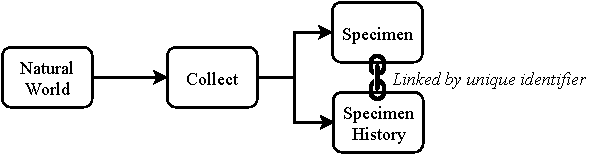
\includegraphics[scale=1]{figures/fig1a.pdf}} \\
\subfigure[Digital data collection]{%
\label{fig:collection-b}%
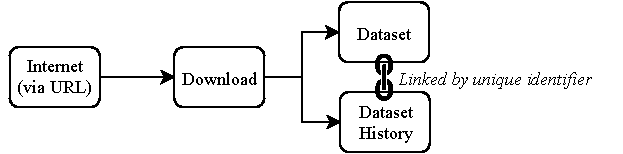
\includegraphics[scale=1]{figures/fig1b.pdf}}%

\caption{Reliable record keeping for digital datasets \subref{fig:collection-b} can be achieved in an analogous way to current practices in record keeping for physical specimens \subref{fig:collection-a}. Biologists collect physical specimens from the natural world, thoroughly document the process, then store the specimens in facilities equipped for long-term preservation. Analogously, digital datasets that are downloaded from the internet can be thoroughly documented and archived in dedicated repositories for long-term preservation. Just as the collection of physical specimens is recorded and identified in specimen history records, the downloading of digital datasets can also be recorded and identified in dataset history records.}%

\label{fig:collection} % \label works only AFTER \caption within figure environment

\end{figure}



The same can be done for downloaded datasets. When a dataset is downloaded, a record can be kept that details the URL that was queried, the time of query, and who (e.g., a human or software agent) issued the query that initiated the download event; we refer to this record as the dataset's provenance record \citep{Pasquier_2017}. Additionally, the dataset itself should be stored in a safe, accessible dataset archive. The final step in the collection process is to link the actual preserved specimen to its corresponding record (see figure \ref{fig:collection-a}) via an assigned unique identifier.

The identifiers assigned to datasets (or provenance data) must differ only if their contents differ. This can be achieved by deriving the identifiers from the content of their respective datasets. Furthermore, the identifier must be unique to the dataset; a dataset will always be assigned the same identifier and no two datasets (including different versions of a dataset) can share an identifier. With these restrictions in place, it is possible to reliably link each recorded dataset to its provenance record without the need for an intermediate index. That is, the derivation of the content-based identifier from a given dataset can be performed by anyone, anywhere, and at any time, without the need to consult some central authority \citep{Paskin_1999}. Cryptographic hashing is one such method for producing content-based identifiers which are both content-derived and unique. A variety of cryptographic hashing algorithms exist that receive some digital file as input and uniquely encode its contents into a fixed-length series of bits called a ``hash.'' We use hashes generated by the SHA-256 algorithm \citepalias{SHA2_2001} as unique content-based identifiers.

\subsection*{Data Collection Over Time}
By establishing a dedicated data observatory that implements the collection process we have described, we can build a history for each observed URL to capture its reliability over time. Such an observatory periodically queries the URLs listed in a data network's URL registry and produces for each URL two complementary parts: 1) an archived copy of the response to the corresponding query, whether it was a dataset, an error code, or no reply at all, and 2) a record of its provenance, including the URL itself, the current date, and a content-based identifier of any dataset received. Successive provenance records can be aggregated to construct comprehensive histories for both datasets (when and where they were found) and URLs (which datasets they located over a series of queries over time).

The constructed URL histories can be analyzed to determine whether a link was ever broken, when it was broken, and whether it became responsive again. The logs also identify the content (or lack of content) that a URL located each time it was queried. Any change in the content identifier from one query to the next indicates a change in the content of the dataset. These link breakages and content changes correlate to link rot and content drift, respectively, and allow us to determine the responsiveness, stability, and reliability of each URL over time.

\subsection*{Data Network Reliability}
Our method for monitoring the behavior of a single URL over time can be applied to observe all URLs registered in a biodiversity data network. We also extend the idea of URL reliability to entire data networks and propose that the overall reliability of a data network can be evaluated by monitoring the reliability of each URL in the network over time. First, we label individual URLs with binary indicators of responsiveness, stability, and reliability. Next, we grade data networks according to the percentage of registered URLs that are assigned each of the reliability indicators. For example, if a data network contains three distinct URLs and we find that only two out of the three are reliable, then we say the data network is 67\% reliable.

\subsection*{Experiment}
The Preston biodiversity dataset tracker \citep{jorrit_poelen_2018_1410543} implements mechanisms for monitoring data networks as we have described. It allows users to deploy a data network observatory, that tracks the entire set of URLs registered in the network, queries each URL for data, then documents data collection and archives the results. All crawl activities, the queries they issue, and the results they produce are recorded in a string of provenance logs.

We deployed several Preston observatories that periodically queried the registered dataset URLs listed by Biodiversity Heritage Library (BHL), Data Observation Network for Earth (DataONE), Global Biodiversity Information Facility (GBIF), and Integrated Digitized Bio Collections (iDigBio). Each of these networks provides online registries of URLs that locate the data in the network. The registered URLs for DataONE, GBIF, and iDigBio were queried monthly from March 2019 through October 2019. BHL was queried monthly from May 2019 through October 2019. The logs taken by each of these observatories describe the URL queries and their results, which were processed to produce the results that follow. A fifth observatory was constructed by aggregating the queries of the four data network observatories.

% uncomment for inline figures
% 
\begin{figure}[t!] %s state preferences regarding figure placement here

% use to correct figure counter if necessary
%\renewcommand{\thefigure}{2}

\centering
\subfigure[BHL]{%
\label{fig:network-reliability-a}%
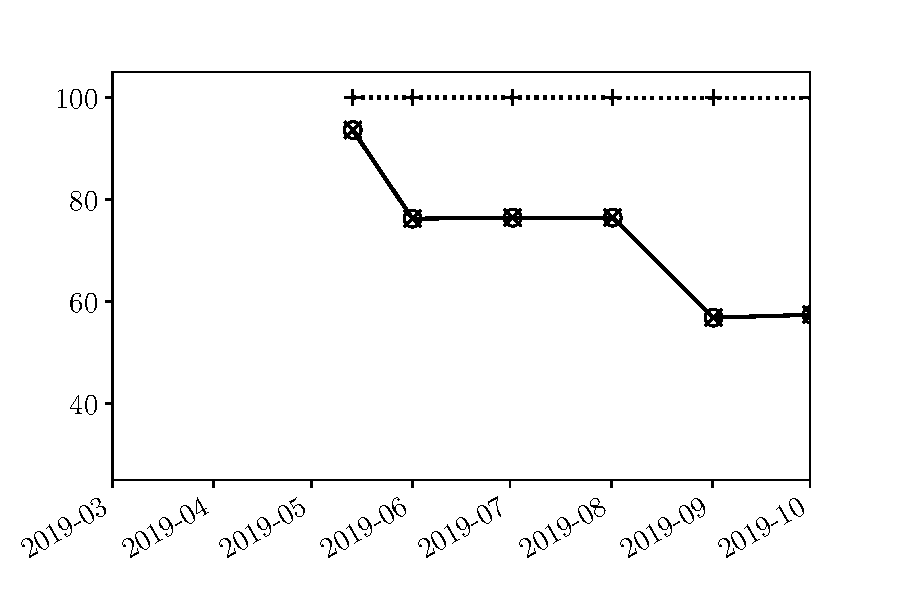
\includegraphics[width=0.5\textwidth]{figures/fig2a.pdf}}%
\subfigure[DataONE]{%
\label{fig:network-reliability-b}%
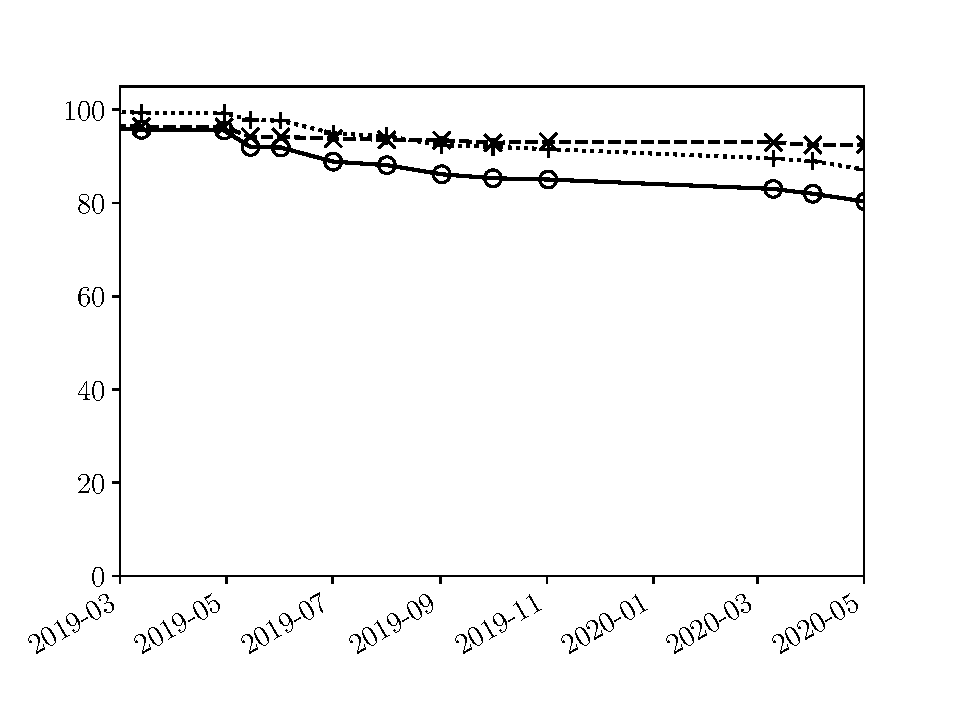
\includegraphics[width=0.5\textwidth]{figures/fig2b.pdf}} \\
\subfigure[GBIF]{%
\label{fig:network-reliability-c}%
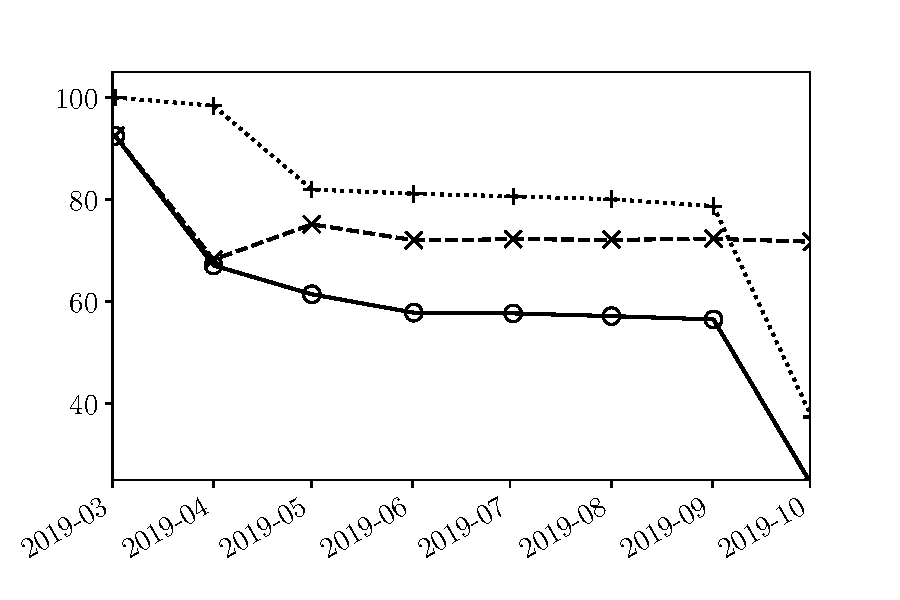
\includegraphics[width=0.5\textwidth]{figures/fig2c.pdf}}%
\subfigure[iDigBio]{%
\label{fig:network-reliability-d}%
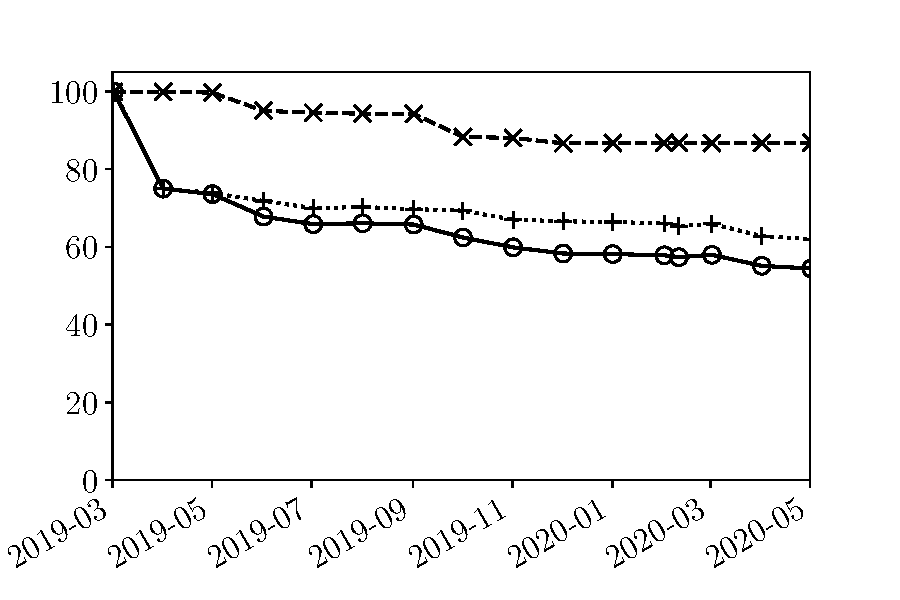
\includegraphics[width=0.5\textwidth]{figures/fig2d.pdf}} \\
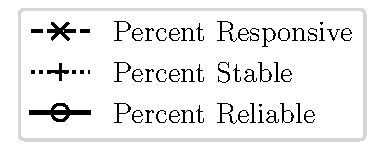
\includegraphics[scale=0.6]{figures/fig2legend.pdf}%

\caption[Network reliabilities over time]{Overall responsiveness, stability, and reliability from March 2019 through October 2019 as percentages of URLs that exhibit each indicator in \subref{fig:network-reliability-a} BHL, \subref{fig:network-reliability-b} DataONE, \subref{fig:network-reliability-c} GBIF, and \subref{fig:network-reliability-d} iDigBio.
}%

\label{fig:network-reliability} % \label works only AFTER \caption within figure environment

\end{figure}





\section*{Results}
\label{sec:results}
Breakdowns of the overall reliabilities of the data networks are provided in table 1. Results are listed as percentages and total counts of URLs in the data network that were assigned each reliability indicator. When analyzing the recorded results of queries to URLs in each data network, we found that, for each individual network, 5\% to 43\% of registered URLs were intermittently or consistently unresponsive, 0\% to 63\% produced unstable content, and 13\% to 76\% became either unresponsive or unstable over the period of observation.

We found that 30\% of URLs observed across the four networks became unreliable at some point over the period of observation. Of those unreliable URLs, 48\% were unstable, 22\% became consistently unresponsive, and 70\% were at best only intermittently responsive. For 5\% of successful queries, the URL failed to respond to the next query. For 4\% of successful queries, the URL provided different content the next time it responded when queried.

The changes in reliability over time for each network are visualized in figure \ref{fig:network-reliability}. Note that because we have defined reliable URLs to be those considered both responsive and stable, they always represent the smallest fraction of URLs in table \ref{table1}, figure \ref{fig:network-reliability}, and figure \ref{fig:network-growth}. Figure \ref{fig:network-growth} visualizes the cumulative growth of biodiversity data networks during their periods of observation. This growth is illustrated with two metrics: the total number of unique URLs ever registered in each network and the total number of unique contents that were downloaded from the network at each monthly sampling.

% uncomment for inline figures
% \begin{figure}[t!] %s state preferences regarding figure placement here

% use to correct figure counter if necessary
%\renewcommand{\thefigure}{2}

\centering
\subfigure[BHL]{%
\label{fig:network-growth-a}%
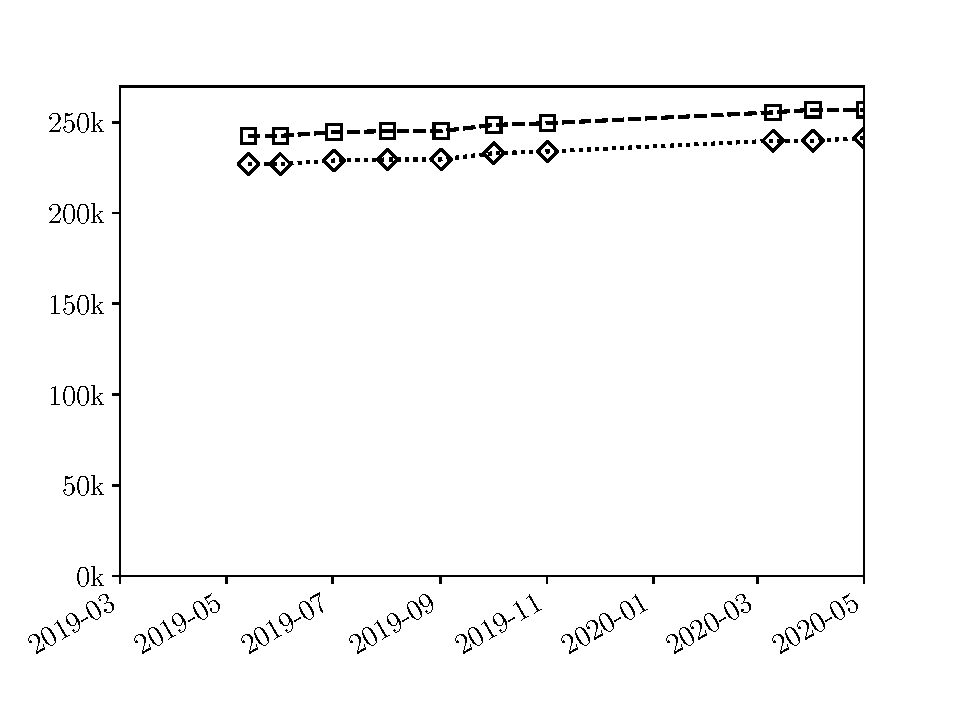
\includegraphics[width=0.5\textwidth]{figures/fig3a.pdf}}%
\subfigure[DataONE]{%
\label{fig:network-growth-b}%
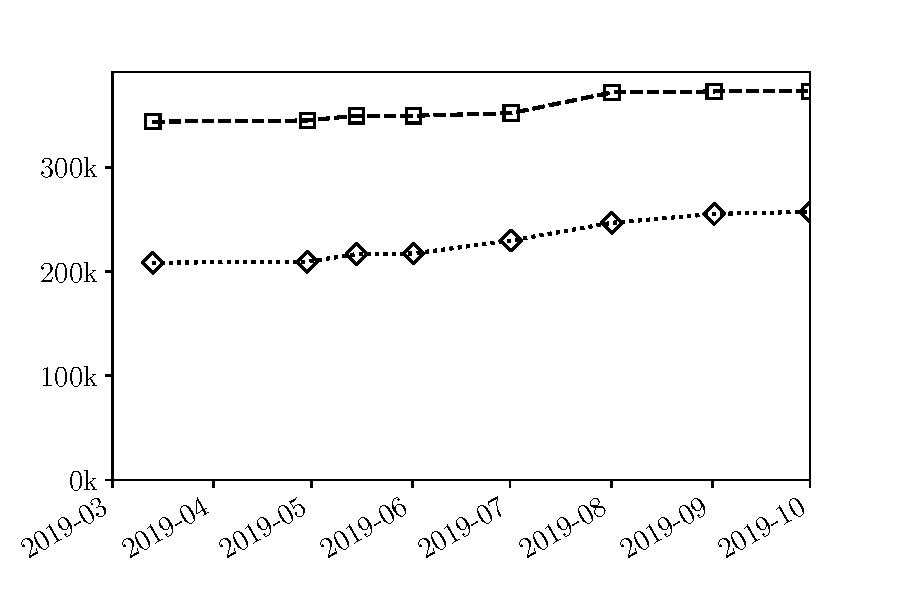
\includegraphics[width=0.5\textwidth]{figures/fig3b.pdf}} \\
\subfigure[GBIF]{%
\label{fig:network-growth-c}%
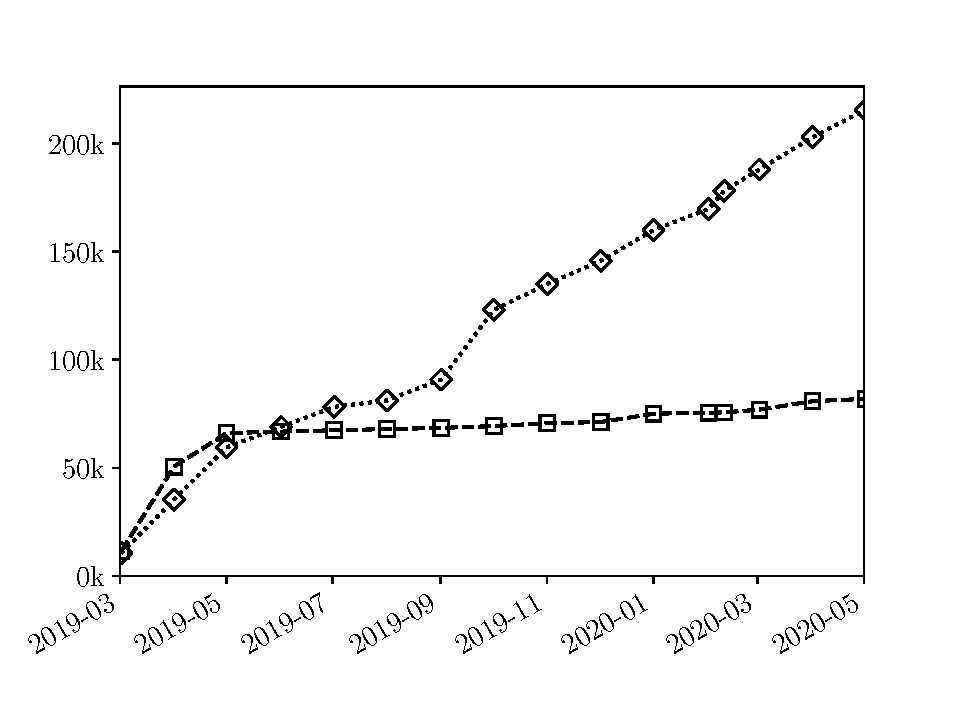
\includegraphics[width=0.5\textwidth]{figures/fig3c.pdf}}%
\subfigure[iDigBio]{%
\label{fig:network-growth-d}%
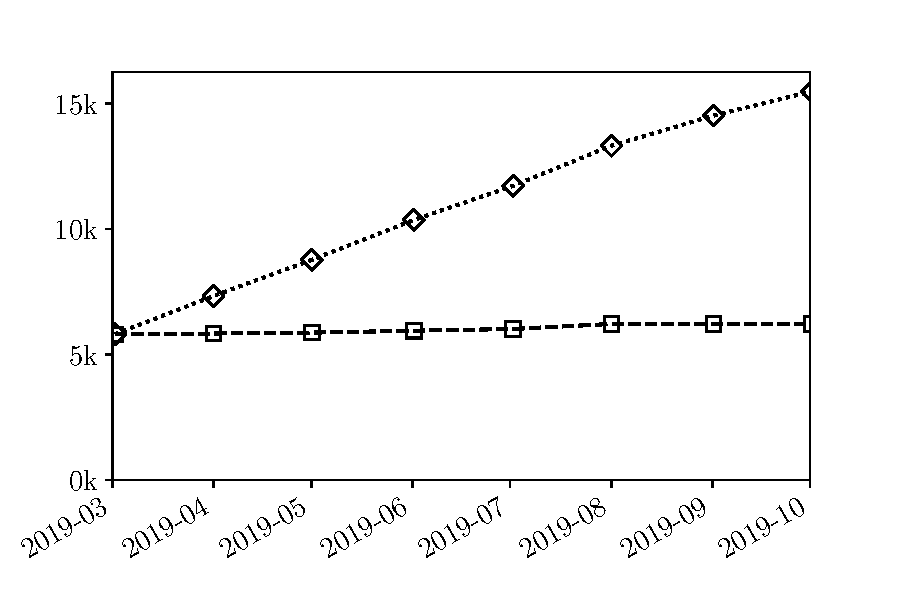
\includegraphics[width=0.5\textwidth]{figures/fig3d.pdf}} \\
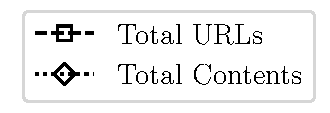
\includegraphics[scale=0.6]{figures/fig3legend.pdf}%

\caption[Network URL and content counts over time]{Total number of URLs and unique contents observed from March 2019 through May 2020 in the provider networks of \subref{fig:network-growth-a} BHL, \subref{fig:network-growth-b} DataONE, \subref{fig:network-growth-c} GBIF, and \subref{fig:network-growth-d} iDigBio.
}%

\label{fig:network-growth} % \label works only AFTER \caption within figure environment

\end{figure}




% uncomment for inline tables
% \begin{table}[!ht]
\begin{adjustwidth}{0in}{0in} % comment out/remove adjustwidth environment if table fits in text column.
\centering
\begin{tabular}{llll}
\hline
{\bf Data Network} & {\bf Responsive URLs} & {\bf Stable URLs*} & {\bf Reliable URLs} \\ \hline
BHL\textsuperscript{a} & 57.41\% (142,672) & 99.97\% (232,996) & 57.39\% (142,633) \\
DataONE\textsuperscript{b} & 94.55\% (352,438) & 92.27\% (339,109) & 87.09\% (324,641) \\
GBIF\textsuperscript{c} & 71.72\% (49,707) & 37.35\% (20,094) & 24.05\% (16,669) \\
iDigBio\textsuperscript{c} & 88.04\% (5,477) & 68.69\% (4,251) & 61.68\% (3,837)  \\
All observed URLs** & 78.94\% (546,645) & 90.43\% (593,469) & 70.07\% (485,203) \\ \hline
\end{tabular}
\caption{Overall responsiveness, stability, and reliability for URLs observed in each biodiversity data network and for all observed URLs as of October 2019.
*URLs that never provided content were omitted from the divisor when calculating Stable URLs percentages.
**Because URLs may be registered in more than one data network, the total number of observed URLs is expected to be less than the sum of the URL counts for each network.
\textsuperscript{a}\citet{poelen_jorrit_h_2019_3484555}
\textsuperscript{b}\citet{poelen_jorrit_h_2019_3483218}
\textsuperscript{c}\citet{poelen_jorrit_h_2019_3484205}
}
\label{table1}
\end{adjustwidth}
\end{table}


The behaviors of the distributions over time of responsive, stable, and reliable URLs vary notably between data networks. Reasons for these differences might be inferred when cross-examining table \ref{table1} and figures \ref{fig:network-reliability} and \ref{fig:network-growth}. For example, although BHL scored relatively low in responsiveness due to frequent link rot, the content that it does provide is more stable than all other networks because content drift within BHL is relatively rare. Conversely, although iDigBio is relatively responsive, it has low stability because the network's near-constant content growth far outpaces its URL growth. GBIF's behavior was characterized by large sporadic swings; a mass URL migration of over 14,000 Plazi-hosted datasets occurred in May, introducing thousands of new URLs over a short period of time, while over 31,000 URLs (60\% of URLs that responded to queries that month) suddenly changed contents in October. Even the most reliable network, DataONE, shows a clear downward trend in all three categories, with 13\% of URLs becoming unreliable over a period of just seven months. Additionally, DataONE's growth curves indicate that there are far fewer unique contents than unique URLs. This mismatch suggests two possibilities: either much of DataONE's URL population is unresponsive, or DataONE lists multiple URLs for many of its datasets. Because DataONE has been shown to be highly responsive, it could be the case that many distinct URLs refer to the same datasets. It's also worth noting that the June and September spikes in BHL's unresponsiveness were largely due to URLs that failed to respond in those particular months but did respond to future queries.

\subsection*{Sources of Potential Numerical Error}
We expect that the URL reliability counts generated for the figures and tables are lower than their actual values. When we qualified URLs as being reliable, responsive, and stable, we could not be certain that links did not briefly become unresponsive or change content during the month-long periods between queries. It is therefore likely that some cases of link rot and content drift were not reflected in the results. Additionally, we only queried URLs that the data networks list in their dataset registries; this means that, if a URL were removed from a network's registry, would not be able to detect subsequent instances of reference rot. Therefore, our results represented an optimistic upper bound on URL and network reliabilities.

The results for DataONE and GBIF in figure \ref{fig:network-reliability} are sometimes skewed due to the pagination method that the networks use to supply users with their dataset registries. Registry pages contained set amounts (e.g., 20) of URLs and represent small slices of the actual data network registry. For registries that use pagination, the observatory would keep querying for registry pages until reaching the page or failing to get a response. For instance, GBIF's URL and dataset totals in March 2019 (see figure \ref{fig:network-growth-c}) are low because an early query to a GBIF registry page was not answered and, consequently, the URLs of registry pages that should have followed were not discovered. Similar events happened for both the GBIF and DataONE observatories at later points in time, potentially overestimating the reliability of the data network.

In an effort to minimize artificial link rot due to internet access issues in our local network, we deployed the Preston observatories in a large commercial data center in Germany.



\section*{Discussion}
We have shown that the reliability of URLs decreases over time in all of the major biodiversity data networks that we monitored. If current trends continue, the extent of reference rot will worsen. Systematic changes in the way we preserve and reference data are needed to reverse these trends and improve the longevity and long-term integrity of the biodiversity data record. Before we propose such changes, it's necessary to first understand why URLs are proving to be ill-suited for referencing data in the long term.

\subsection*{Unreliability of Location-Based Identifiers}
The problems related to using URLs for referencing datasets are largely due to the fact that they are location-based identifiers: they describe where the data is but not necessarily what it is. Also, by definition, data accessed via URLs must be mediated by a central authority, such as the institutional repositories that serve biodiversity datasets, who can match location-based identifiers with data. Interested users are expected to trust the central authority to guarantee long-term access to the referenced data in its original form.

The use of URLs as identifiers violates the requirements of uniqueness and persistence \citep{Paskin_1999}. An identifier must only ever identify one entity (uniqueness) and must persist longer than the entity it identifies (persistence) \citep{Paskin_1999}. However, as we have shown in our experiments, many URLs do not possess both uniqueness and persistence; unstable URLs forfeit uniqueness in the event of content drift, while unresponsive URLs do not persist as long as the datasets they identify.

At the core of URL instability is the current practice of using URLs to identify evolving datasets rather than fixed dataset versions. If biodiversity data providers were uniformly committed to allocating one URL per dataset version, then content drift might  become less common, improving overall URL stability; however, widespread social adoption of such a commitment from all data providers may be unrealistic. Additionally, such a commitment would not address link rot and URL unresponsiveness. Even if a similar commitment were made by data providers to guarantee the long-term responsiveness of URLs, it could not address the case where a data provider either loses authority over a domain name or migrates to another. For example, our deployed Preston observatories recorded the sudden migration of over 14,000 Plazi datasets from the http://plazi.cs.umb.edu/ domain to http://tb.plazi.org/, an event which invalidated any references to URLs within the first domain.

Paskin proposed that ``the best way to `future proof' an identifier scheme is to forego any intelligence within the identifier itself'' \citep{Paskin_1999}, where the notion of intelligence refers to the inclusion of meaningful information in the textual representation of the identifier. URLs are typically structured according to the Domain Name System specification (though URLs may include an IP address instead of a domain name) and inherently contain some minimum amount of intelligence, namely the domain to which the URL belongs \citep{rfc1034}. Thus, it is necessary to look to another identification scheme to allow for proper identification and reliable referencing.

\subsection*{An Alternative: Unique Content-Based Identifiers}
Instead of identifying digital datasets by location (e.g., a URL), we can identify datasets by their content. One way to achieve this is to use algorithmically generated content-based identifiers. A variety of cryptographic hashing algorithms are available that guarantee a unique hash, representable as text, for any given dataset \citepalias{SHA2_2001}. Because the hash is deterministically derived from the content it identifies, we say that it is a content-based identifier. These content-based identifiers can be generated for a dataset using openly available algorithms, without a mediating central authority \citep{Paskin_1999}. If a change is made to the dataset, then the hash computed from the modified dataset will be different from that of the original. Therefore, if the hash of a dataset is the same as the referenced hash, it must be the originally referenced dataset (figure \ref{fig:verification-c}) \citepalias{SHA2_2001}. Using hash identifiers eliminates the possibility of content drift.

% Introduce repositories vs registries

The shift from location-based to content-based identifiers decouples future dataset accessibility from the original point of access. As long as there exists some discoverable and accessible data repository that serves the desired content, that content can always be retrieved. Such data repositories can be made discoverable through content hash registries such as hash-archive.org \citep{Trask_2015}. In response to a user query for a content hash, these content hash registries would provide a list of locators (e.g., URLs), if any, that direct users to the referenced data (e.g., a registry would provide URLs that retrieve data when queried). Even if one repository becomes inaccessible due to either a temporary outage or permanent retirement, another may be available to provide the referenced data. When several repositories serve referenced datasets, there is no single point of failure for content hash lookups; if a referenced dataset is redundantly located across and within data repositories, access to the dataset will only be lost if all associated locations exhibit link rot. Even if access to a dataset is lost, it can be restored as long as the referenced dataset still exists somewhere and can be made discoverable and accessible.

If a dataset version were identified with a content-based hash, its duplication across different platforms would not lead to ambiguous references, but rather to distributed copies of the same reliably addressed content.

% uncomment for inline figures
% \begin{figure}[!p] %s state preferences regarding figure placement here

% use to correct figure counter if necessary
%\renewcommand{\thefigure}{2}

\centering
\subfigure[URL reference]{%
\label{fig:verification-a}%
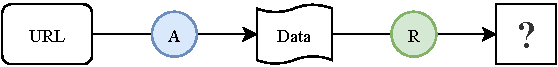
\includegraphics[scale=0.74, right]{figures/fig4a.pdf}} \\
\subfigure[URL reference with content hash]{%
\label{fig:verification-b}%
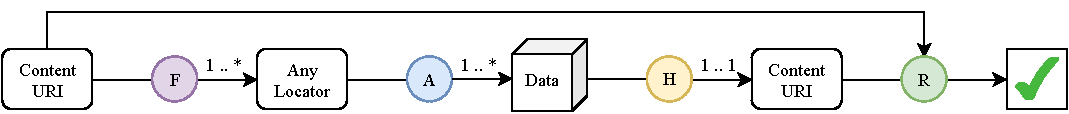
\includegraphics[scale=0.74, right]{figures/fig4b.pdf}} \\
\subfigure[Content URI reference]{%
\label{fig:verification-c}%
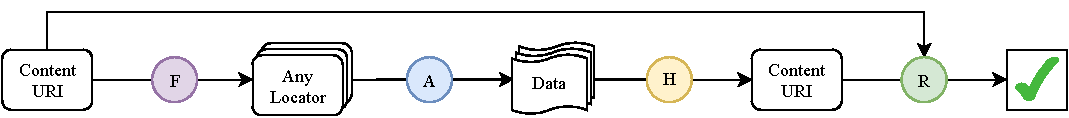
\includegraphics[scale=0.74, right]{figures/fig4c.pdf}} \\
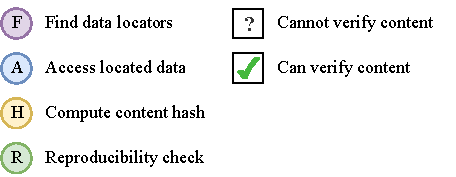
\includegraphics[scale=.9]{figures/fig4legend.pdf}%

\caption{Content resolution and verification for references that use location- versus content-based identifiers. \subref{fig:verification-a} Location-based identifiers (e.g. URLs) cannot verify the authenticity of retrieved content and are vulnerable to link rot due to the use of a fixed locator. \subref{fig:verification-b} If the content hash of the referenced data is known, the authenticity of retrieved data can be verified by comparing the hash of the retrieved data with the provided content hash. However, the fixed locator is still vulnerable to link rot. \subref{fig:verification-c} Content-based identifiers (e.g. Content URIs) can be used to find several locators for the referenced data and contain a content hash to verify the authenticity of retrieved data. The decoupling of the reference from a fixed locator makes the reference resistant to link rot.
}%

\label{fig:verification} % \label works only AFTER \caption within figure environment

\end{figure}


\subsection*{Transitioning to Reliable References}
Although we propose a change in the fundamental mechanisms used to reference datasets, existing references can be made reliable with only minor modifications. Consider the following citation generated by GBIF according to their citation guidelines \citepalias{gbif_2019}:

\begin{quote}
Levatich T, Padilla F (2017). EOD - eBird Observation Dataset. Cornell Lab of Ornithology. Occurrence dataset https://doi.org/10.15468/aomfnb accessed via GBIF.org on 2018-09-02.
\end{quote}

The citation references the eBird dataset hosted at gbif.org as it was retrieved on September 2, 2018. However, at the time of writing, the URL https://doi.org/10.15468/aomfnb redirects to a GBIF internal reference page that states the eBird dataset was last updated in March of 2019. The dataset made available through the listed URL is different from what was originally referenced in the citation, but it is impossible to determine the extent of the changes without having access to previous versions of the data.

Fortunately, references like the example above can be made more reliable by augmenting them with a content-based identifier for the dataset. Consider the following enriched citation for the eBird dataset that adds a SHA-256 content hash \citepalias{SHA2_2001}:

\begin{quote}
Levatich T, Padilla F (2017). EOD - eBird Observation Dataset. Cornell Lab of Ornithology. Occurrence dataset \seqsplit{hash://sha256/29d30b566f924355a383b13cd48c3aa239d42cba0a55f4ccfc2930289b88b43c} accessed at https://doi.org/10.15468/aomfnb via GBIF.org on 2018-09-02.
\end{quote}

The content hash is captured in a content address Uniform Resource Identifier (URI) \citep{rfc3986} in the form of hash://algo/hash-string proposed by \citep{Trask_2015}, where ``algo'' is a hashing algorithm (e.g., ``sha256'') and ``hash-string'' is the content hash generated by the algorithm in hexadecimal format. In the example above, the hashing algorithm is SHA256 and the hash string starts with ``29d3.'' The added content hash was derived from and uniquely identifies the exact version of the eBird dataset that was originally referenced. If an interested user knows of and has access to an information retrieval system that has indexed the dataset, finding the desired dataset is as simple as querying for its content hash. With the addition of a content hash, the URL becomes superfluous and is included merely to demonstrate that the URL and content hash are not mutually exclusive (see figure \ref{fig:verification-b}).

Note that different hashing algorithms will generate different content hashes from the same data. We use a URI rather than the content hash itself because it allows us to specify the hashing algorithm. If the hashing algorithm is not specified, one might mistakenly conclude that a dataset does not match a reference if the wrong hashing algorithm is used to verify the dataset's authenticity. Our proposal to use Trask's content-addressed URIs to reliably reference data is inspired by Kuhn \& Dumontier's method to make digital content verifiable and permanent using Trusty URIs \citep{Kuhn_2015}. We chose to use Trask's content hash URIs because they are location- and content-agnostic and easy to read. However, we recognize that Trusty URIs can help facilitate content retrieval and processing using a location-based URI prefix and an (optional) extension suffix.

Other content-based identification schemes exist that resist changes in format in digital content. For example, the universal numeric fingerprint (UNF) \citep{Altman_2007} resists such changes by first processing the input data before generating a content hash. Among other preprocessing techniques used when generating UNFs, numerical data may be rounded to a certain precision before generating a content hash, with the understanding that a dataset may undergo such format changes when translated, for example, between different computing envirionments or hardware configurations. Indeed, on manual examination of the changes between successive versions of the biodiversity datasets we observed, we found some cases in which two versions of a dataset (determined to be different because they resulted in different content hashes) differed only in formatting, such as the amount of whitespace and the sequential ordering of observational records. However, for biodiversity data, we expect that such format-specific content-based identification schemes would only prove detrimental in practice. Standard cryptographic hashing algorithms, such as SHA-256, are included in most modern software environments and enjoy widespread use across different digital applications, whereas non-standard algorithms, such as UNF, would first need to be installed and may be unknown to most users, presenting a hurdle to their widespread adoption. Additionally, it may be unrealistic to expect preprocessing efforts to filter out non-informative data effectively enough to be able to trust that semantically identical datasets will always result in the same content-based identifiers. This is especially relevant to biodiversity datasets because they consist mostly of text data, which may be altered in a number of ways without changing the content’s meaning.

\subsection*{Enhancing Dataset References with Provenance}
A dataset reference can also be enhanced by pointing to the record that describes its provenance. The following citation further augments the eBird dataset reference with the content hash of an associated provenance record:

\begin{quote}
Levatich T, Padilla F (2017). EOD - eBird Observation Dataset. Cornell Lab of Ornithology. Occurrence dataset \seqsplit{hash://sha256/29d30b566f924355a383b13cd48c3aa239d42cba0a55f4ccfc2930289b88b43c} accessed at https://doi.org/10.15468/aomfnb via GBIF.org on 2018-09-02 with provenance \seqsplit{hash://sha256/b83cf099449dae3f633af618b19d05013953e7a1d7d97bc5ac01afd7bd9abe5d}.
\end{quote}

As was the case for the dataset, the provenance itself can be retrieved by querying an information system that has indexed the hash of the referenced provenance record. Note that the provenance hash is not strictly necessary to make a dataset reference reliable; the dataset hash alone is sufficient. However, explicitly referencing the provenance of the dataset is useful because it allows future readers to retrieve the same context to which the researcher referencing the dataset had access. More generally, the provenance describes the context of the retrieval of any type of content (e.g., datasets, metadata, citation files, etc.). The types of information in the provenance depend on the implementation of the data observatory, but at a minimum include the URLs that were queried to produce the content, the dates of the queries, the format of the content, and the data registries that were searched to find the content.

% uncomment for inline figures
% \begin{figure}[t] %s state preferences regarding figure placement here

% use to correct figure counter if necessary
%\renewcommand{\thefigure}{2}

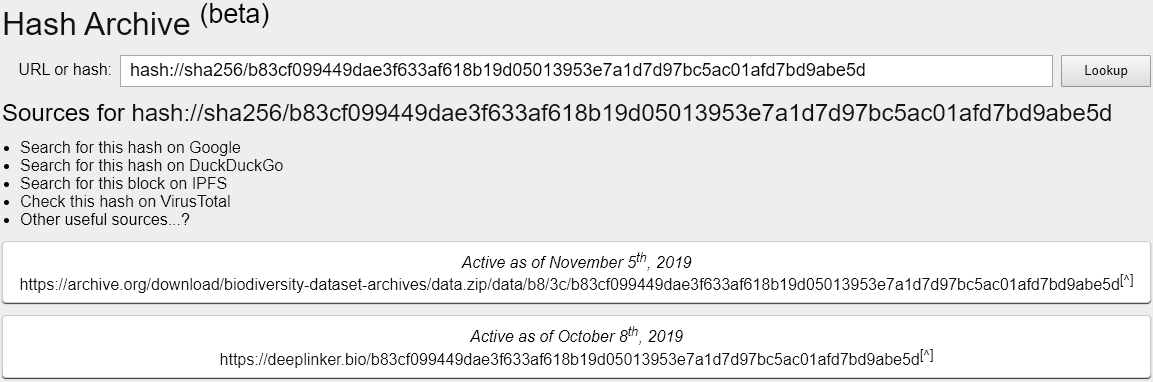
\includegraphics[width=\textwidth]{figures/fig5_grayscale.png}

\caption{An example of a search index mapping hashes to archives. A search for a content or provenance hash at hash-archive.org will find any associated URLs that have been registered at hash-archive.org.}

\label{fig5} % \label works only AFTER \caption within figure environment

\end{figure}


The use cases for including the provenance hash are many. For example, if the provenance record of a dataset is found, it may be possible to traverse the provenance and find newer versions of the dataset. This requires that the various versions of the dataset were observed by a provenance-generating data observatory, properly archived, then made publicly accessible.

A provenance record relates to a dataset the way that a map relates to a location: a provenance record provides a context to understand the origin and relations of a dataset. This provenance context may be limited to few metadata elements related to a single dataset (e.g., web location, data format, author, license), but can also include a comprehensive description of a biodiversity dataset network consisting of thousands of datasets and their associations. Also, because provenance records are datasets themselves, they can be reliably referenced and embedded in other provenance records using their content URIs. We used such a composition of content URIs and provenance records as part of our monitoring scheme \citep{jorrit_poelen_2018_1410543} to track the reliability of URLs in biodiveristy data networks over time (see table \ref{table1} and figures \ref{fig:network-reliability} and \ref{fig:network-growth}). The following citation references the history of the entire DataONE network over the period of observation by one of our Preston observatories:

\begin{quote}
Poelen JH. 2019d. A biodiversity dataset graph: DataONE.
doi:10.5281/zenodo.3483218 . \seqsplit{hash://sha256/87de0898919d2212977a586965e930ae45bdd1366073591c808c208a635e2814}
\end{quote}

\subsection*{Dataset Retrieval Using Hash References}
The dataset and provenance hashes referenced in the sample references above were produced by our Preston observatories, which were set up to monitor the four data networks. Both the referenced dataset and its provenance are available online at zenodo.org \citep{poelen_jorrit_h_2019_3483218, poelen_jorrit_h_2019_3484555, poelen_jorrit_h_2019_3484205} and archive.org \citep{poelen_jorrit_h_2019_archive_org}. A query for the provenance hash in the search bar at zenodo.org or hash-archive.org should direct the user to an archived repository of Preston observations that contains both the dataset and its provenance (see figure \ref{fig5}). Given Zenodo's long-term guarantee for data persistence and version availability \citep{zenodo_2019}, the dataset reference is now reliable; it is effectively immune to both link rot and content drift. Future readers can trust that the dataset will stay available and, when downloaded, identically match the version of the eBird dataset we referenced. Note that, to comply with Zenodo's limitations on user uploads \citep{zenodo_2019}, we only exposed the set of provenance hashes collected by each deployed Preston observatory for search indexing, which are far fewer in number than the dataset hashes. Thus, a query to zenodo.org for the dataset hash above should not produce any results. This is an artificial limitation; ideally, an information system would index the dataset hashes as well. Note that our Zenodo publication for the GBIF/iDigBio/BioCASe observatory \citep{poelen_jorrit_h_2019_3484205} contains only provenance, although the Internet Archive publication \citep{poelen_jorrit_h_2019_archive_org} contains the content as well as provenance. Our Zenodo and Internet Archive publications for BHL \citep{poelen_jorrit_h_2019_3484555, poelen_jorrit_h_2019_archive_org_bhl} and DataONE \citep{poelen_jorrit_h_2019_3483218,poelen_jorrit_h_2019_archive_org_dataone} contain both content and provenance.

Several biodiversity data aggregators, such as GBIF and iDigBio, produce a citation file for each user query to allow researchers to simply reference a single citation file rather than each individual dataset \citepalias{gbif_2019,idigbio_2016}. A citation file lists the URLs, attributions, and retrieval dates of the datasets that were returned by a query. We have demonstrated that dataset URLs are unreliable references; thus, citation files that rely on URLs as references are also unreliable. Citation files could be made reliable if they were augmented with the hashes of the retrieved datasets and, optionally, their provenance records. In fact, citation files themselves can be referenced by hash, along with accompanying provenance hashes, as long as they are archived and made accessible.

\subsection*{DOIs for Datasets and Queries}
Biodiversity data aggregators often assign each dataset or query a Digital Object Identifier (DOI) \citep{Paskin_2009} (e.g., 10.123/456) wrapped as a URL (e.g., https://doi.org/10.123/456) and advise researchers to reference the generated DOI rather than a URL. Unfortunately, this abstraction does little to enhance the reliability of the reference.

The DOI Handle System \citep{Paskin_2009} associates DOIs with online resources. However, it does not enforce any constraint on type of resource associated with a DOI. When DOIs are used to reference biodiversity datasets, the associated resources are often URLs, and therefore the use of such DOIs can be as unreliable as using URLs. In practice, these DOIs identify the evolving dataset (or set of datasets in the case of a query) rather than a fixed version, as demonstrated in the example references above. It is possible that an author would wish to make such a reference to an evolving online digital object. For example, an author promoting use of a published dataset might want future users to be directed to the most up-to-date content. However, such a fluid reference is not appropriate for making published results reproducible.

The Handle System allows for a complex web of redirection and distributed responsibilities. Just as the Domain Name System resolves domain names in URLs to IP addresses, the DOI Handle System allows DOIs to be resolved to URLs. However, the responsibility for resolving DOIs to URLs is divided between the Handle System and DOI registrars. The Handle System serves as the central authority that maps DOI prefixes to DOI registrars, examples of which include BHL, DataONE, and GBIF. These registrars are responsible for associating DOIs that match their designated prefix with URLs, and are free to change the URL associated with any given DOI under their jurisdiction \citep{Paskin_2009,DOI_2018}.

The ability of biodiversity data networks to change the URL associated with a DOI is good for reference reliability in the sense that networks can account for dataset migration without compromising existing references. However, the use of DOIs addresses neither the instability of the URLs they redirect to nor cases of link rot in which no URLs remain responsive to serve the referenced dataset. Additionally, as the number of datasets identified online continues to grow, proper maintenance of all of the DOIs a data network administrates might become more unsustainable over time, potentially increasing the risk of unreliable URLs going undetected.

In an article proposing HTTP-URI-based stable identifiers (e.g., URLs that are resolvable over HTTP) for biological collection objects, Güntsch et al. admit that the use of DOIs does not solve the problem of unreliable referencing but merely deflects the burden of URL maintenance onto institutional repositories \citep{G_ntsch_2017}. In contrast, we propose a dataset referencing scheme that is reliable and can be supported by existing infrastructures and workflows. If existing workflows require references to be in the form of DOIs, it could be convenient to embed content hashes into DOIs. Such an approach has already been established for ISBNs through the creation of actionable ISBNs, or ISBN-As \citep{Weissberg_2008}, which may serve as a model for actionable content hashes.

\subsection*{What It Means to Preserve Data}
Our results indicate that reference rot threatens the integrity of published biodiversity datasets. We have seen that the use of content-based identifiers can effectively address the issue of reference rot. However, identifiers are of little use in a vacuum. An identifier can only be useful for data retrieval when combined with a resolver to associate identifiers with locations and a database to retrieve the dataset at the associated location \citep{Paskin_1999}. Thus, we need to address how resolvers and databases might be organized to accommodate content-based identifiers in order to fully realize long-term data preservation. In this context, we define data preservation as the continued capacity for datasets to be reliably referenced and retrieved in their original form even as the global digital biodiversity network evolves over time.

We propose four requirements that must be met to ensure proper data preservation: 1) datasets must be addressable and retrievable using content-based rather than location-based identifiers; 2) an agent must exist to collect datasets, record their provenance, and deposit both to a dedicated repository; 3) these repositories should archive data that could be used in the future; and 4) content hash registries should be openly accessible to resolve hash identifiers to dataset locations within such repositories. Although openly accessible registries should make archived data discoverable, access to those data can still be restricted. Additionally, for the purposes of archiving, it is important that the recorded provenance records do not necessarily describe the datasets themselves, but rather the activities that led to the procurement of those datasets; the primary purposes of provenance in the context of an archive are to document the fact that evidence (i.e., an observation of a dataset) does exist and to make it discoverable for interested users \citep{Bearman_1995}.

We have shown that software agents such as Preston can be used to collect datasets and their provenance over time while maintaining content-addressability; all that is needed to ensure proper data preservation are a dedicated repository and an openly accessible content hash registry to map content-based identifiers to datasets located in the repository. In practice, repositories and registries (and potentially software agents such as Preston deployments) can be co-located; examples include Zenodo and the Internet Archive, although they impose some limitations that may restrict file size, number of files, and the amount of information that can be indexed \citep{zenodo_2019,archive_2019}. These existing information systems may serve as models for long-term biodiversity information systems. These requirements help to ensure that biodiversity data remain FAIR (Findable, Accessible, Interoperable, and Reusable) \citep{Wilkinson_2016}. Findability is achieved through the publishing of provenance logs which thoroughly describe what datasets are and where they originated from. The amenability of the content-based identification paradigm to the operation of independent decentralized repositories strengthens accessibility by preventing the failure of a single data repository from inhibiting future data access (see figure \ref{fig:verification}). Content-based identification also contributes to interoperability across data networks due to the absence of any central authority to administrate data access; a content hash computed from a dataset is guaranteed to match the hash computed by any other agent using the same dataset. Furthermore, content-based identifiers can be embedded in or referenced by DOIs to maintain compatibility with systems that use DOIs as identifiers. Finally, and particularly relevant to this paper's purpose, reusability is strengthened by enhancing the retrievability of referenced datasets and allowing users to verify that a retrieved dataset exactly matches that which was referenced.



\section*{Conclusions}
Although reference rot is resulting in a steady decline in the reliability of our digital biodiversity record, realistic solutions are available to address the root causes of the issue. Content drift can be eliminated altogether by changing the way we reference datasets from using location-based identifiers to ones that are content-based. Meanwhile, the online biodiversity data networks can be made more resilient to link rot if decentralized observation, archival, and distribution techniques are used to capture incremental changes to the data record so that references can remain valid even when online datasets are updated, removed, or relocated. The use of content-based identifiers should be considered by biodiversity data aggregators in order to increase the reliability of references to the data they aggregate.

We have demonstrated that data observatories can be deployed to track the growing digital biodiversity data record. Using the dataset provenance collected over a period of seven months, we were able to quantify the change in reliability over time in terms of link rot and content drift exhibited by the URLs registered in major biodiversity data networks. Even if data networks uniformly adopted content-based identification of datasets and maintained versioned datasets, our method of quantifying link rot and content drift in data networks could be used to monitor whether either of these issues persist in practice due to implementation flaws or non-technical issues.

Biodiversity data observatories can also be used be used to increase the longevity of the biodiversity data record. Such observatories can be used to form reliable dataset references as well as recover datasets that would otherwise become inaccessible due to link rot and content drift. Additionally, the dataset provenance captured by such observatories serves as evidence of the evolution and distribution of the digital biodiversity data record. The combination of archived datasets and provenance can ensure the long-term reproducibility of scholarly works that reference ever-evolving biodiversity datasets.

Furthermore, the establishment of dedicated data repositories and publicly accessible content hash registries are beneficial for making content-addressed biodiversity data discoverable, distributable, and long-lived, by making the datasets and provenance captured by biodiversity data observatories securely archived and publicly available.

Great care has been taken to establish rigorous preservation guidelines for physical specimens, yet there is much that can be done to increase the longevity of our digital data. Our method is not only suited for tracking datasets in biodiversity data networks, but also provides a resilient and reliable way to publish, reference, and preserve scientific digital datasets without having to abandon our existing infrastructures. The method provides a much-needed foundation for constructing digital provenance graphs from an accessible, verifiable, and citable digital scholarly record.

%\clearpage

\section*{Acknowledgments}
The research reported in this paper was funded in part by a grant (NSF OAC 1839201) from the National Science Foundation and the AT\&T Foundation. The authors acknowledge early exchanges with Matt Collins, Anne Thessen, Jen Hammock, Katja Seltmann, and Carl Boettiger.

\nolinenumbers

%This is where your bibliography is generated. Make sure that your .bib file is actually called library.bib
\bibliography{references/biblio}

%This defines the bibliographies style. Search online for a list of available styles.
\bibliographystyle{references/cse}

%--------------------------------------------------------%
%	FIGURES
%--------------------------------------------------------%

% NOTE: If your submission guidelines don't require figures
% at the end, you can comment out the two lines below,
% and embed figures in the text of content.tex instead of here

\newpage
\section*{Figures}
\begin{figure}[ht] %s state preferences regarding figure placement here

% use to correct figure counter if necessary
%\renewcommand{\thefigure}{2}

\centering
\subfigure[Physical specimen collection]{%
\label{fig:collection-a}%
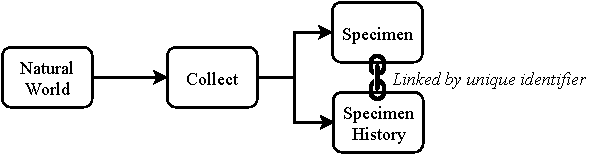
\includegraphics[scale=1]{figures/fig1a.pdf}} \\
\subfigure[Digital data collection]{%
\label{fig:collection-b}%
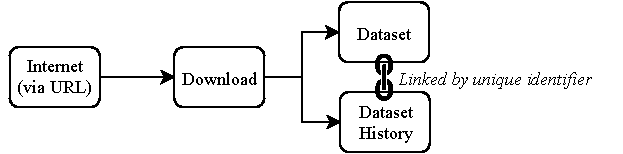
\includegraphics[scale=1]{figures/fig1b.pdf}}%

\caption{Reliable record keeping for digital datasets \subref{fig:collection-b} can be achieved in an analogous way to current practices in record keeping for physical specimens \subref{fig:collection-a}. Biologists collect physical specimens from the natural world, thoroughly document the process, then store the specimens in facilities equipped for long-term preservation. Analogously, digital datasets that are downloaded from the internet can be thoroughly documented and archived in dedicated repositories for long-term preservation. Just as the collection of physical specimens is recorded and identified in specimen history records, the downloading of digital datasets can also be recorded and identified in dataset history records.}%

\label{fig:collection} % \label works only AFTER \caption within figure environment

\end{figure}



\begin{figure}[t!] %s state preferences regarding figure placement here

% use to correct figure counter if necessary
%\renewcommand{\thefigure}{2}

\centering
\subfigure[BHL]{%
\label{fig:network-reliability-a}%
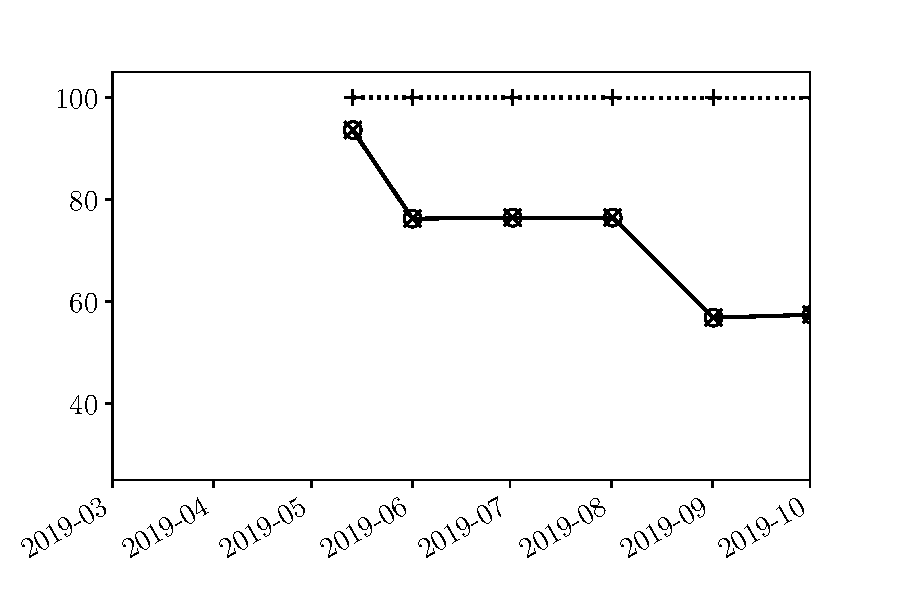
\includegraphics[width=0.5\textwidth]{figures/fig2a.pdf}}%
\subfigure[DataONE]{%
\label{fig:network-reliability-b}%
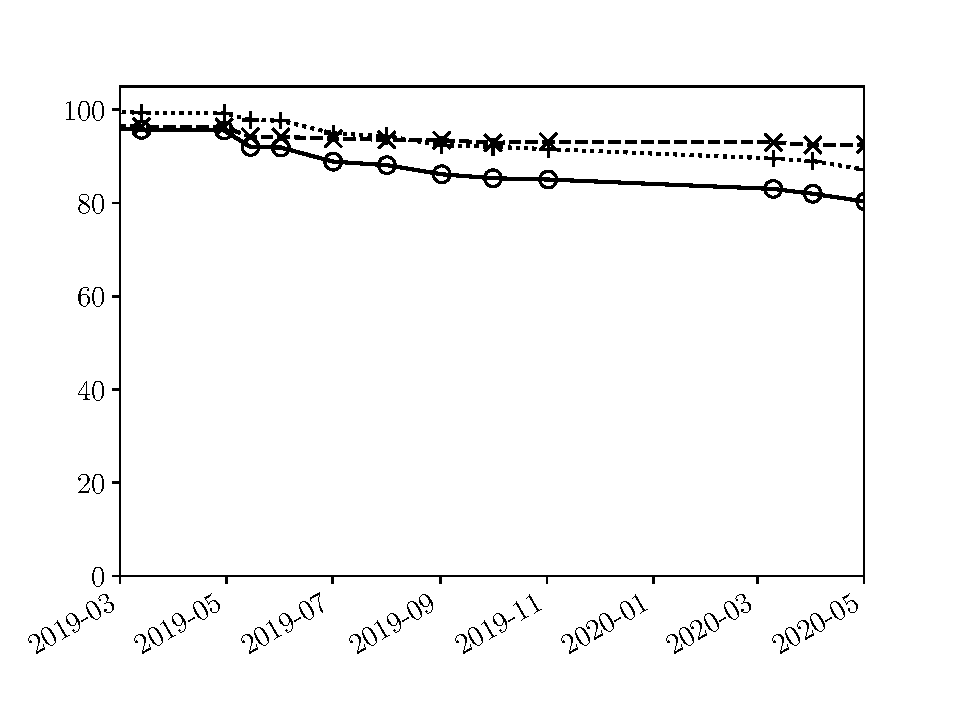
\includegraphics[width=0.5\textwidth]{figures/fig2b.pdf}} \\
\subfigure[GBIF]{%
\label{fig:network-reliability-c}%
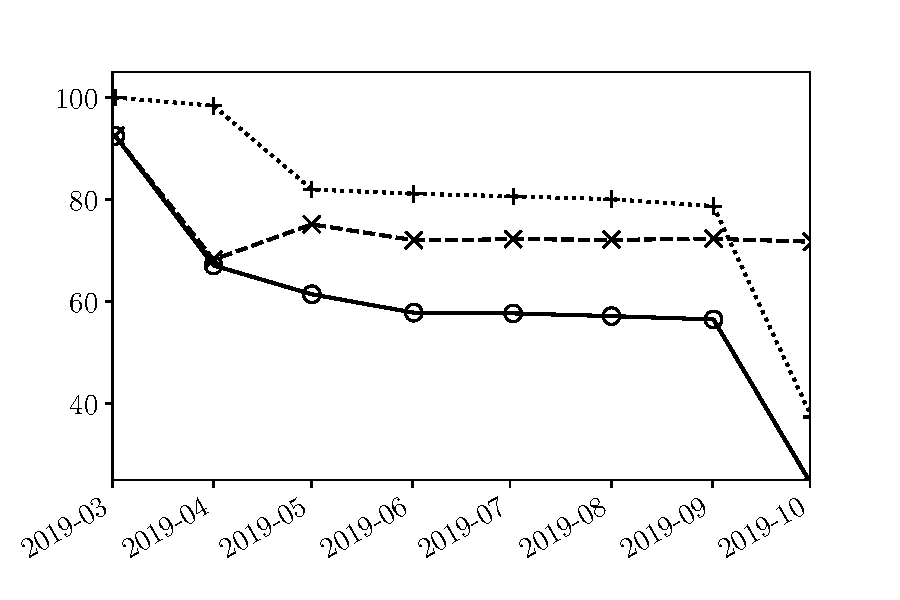
\includegraphics[width=0.5\textwidth]{figures/fig2c.pdf}}%
\subfigure[iDigBio]{%
\label{fig:network-reliability-d}%
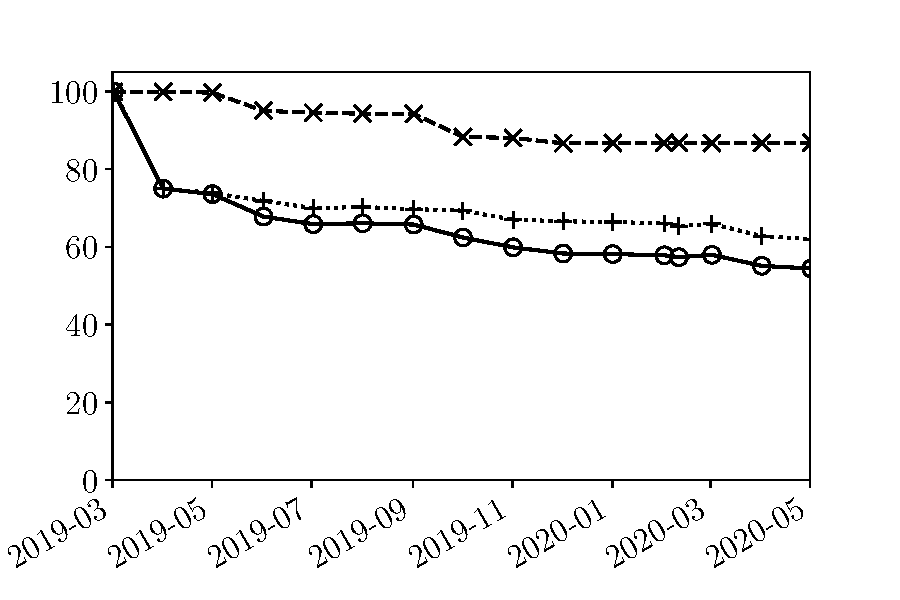
\includegraphics[width=0.5\textwidth]{figures/fig2d.pdf}} \\
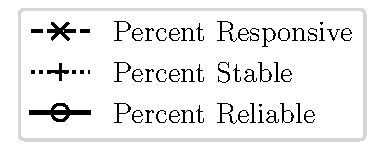
\includegraphics[scale=0.6]{figures/fig2legend.pdf}%

\caption[Network reliabilities over time]{Overall responsiveness, stability, and reliability from March 2019 through October 2019 as percentages of URLs that exhibit each indicator in \subref{fig:network-reliability-a} BHL, \subref{fig:network-reliability-b} DataONE, \subref{fig:network-reliability-c} GBIF, and \subref{fig:network-reliability-d} iDigBio.
}%

\label{fig:network-reliability} % \label works only AFTER \caption within figure environment

\end{figure}


\begin{figure}[t!] %s state preferences regarding figure placement here

% use to correct figure counter if necessary
%\renewcommand{\thefigure}{2}

\centering
\subfigure[BHL]{%
\label{fig:network-growth-a}%
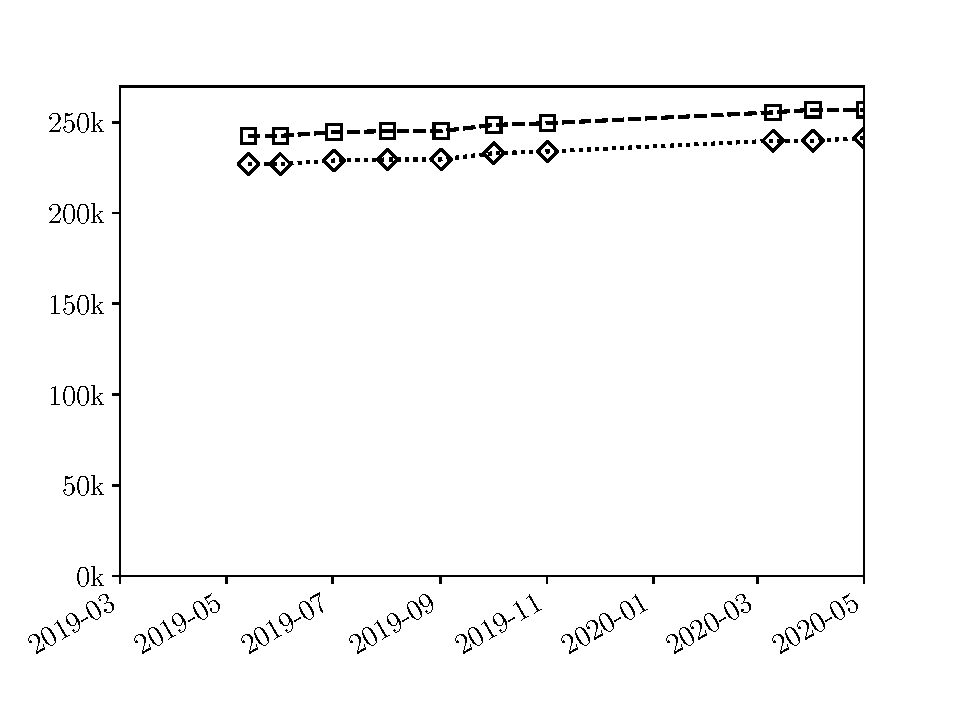
\includegraphics[width=0.5\textwidth]{figures/fig3a.pdf}}%
\subfigure[DataONE]{%
\label{fig:network-growth-b}%
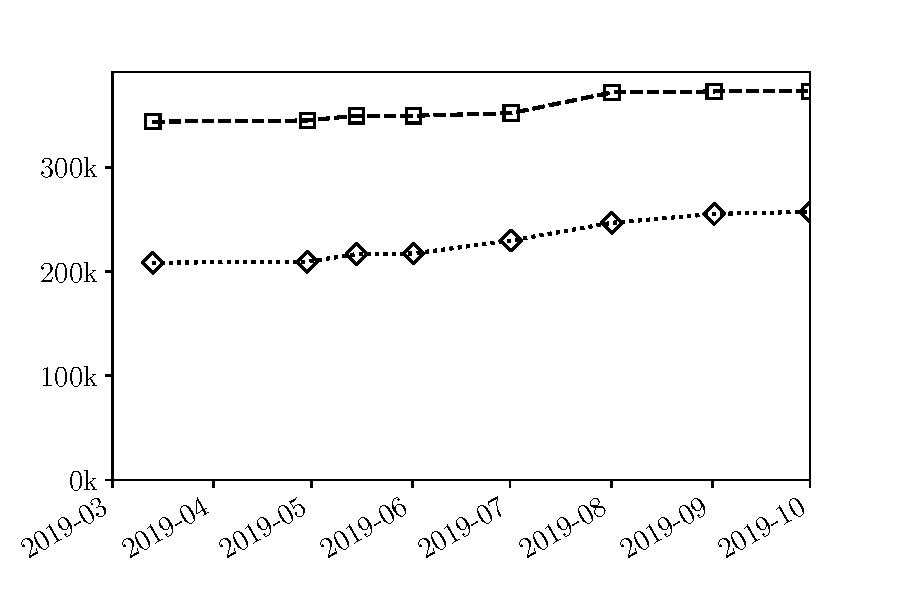
\includegraphics[width=0.5\textwidth]{figures/fig3b.pdf}} \\
\subfigure[GBIF]{%
\label{fig:network-growth-c}%
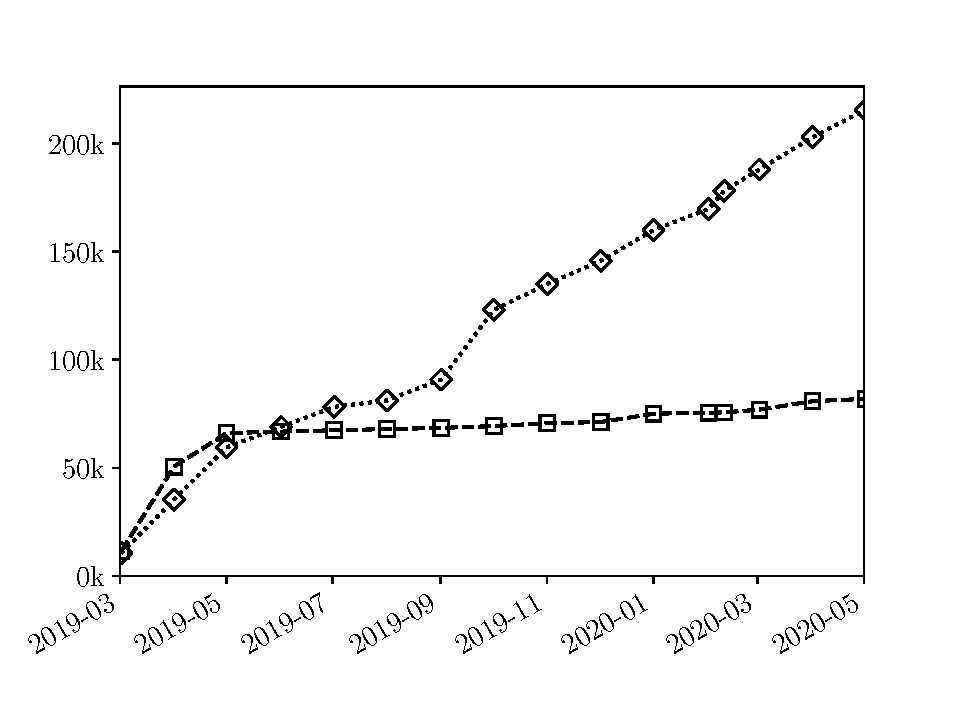
\includegraphics[width=0.5\textwidth]{figures/fig3c.pdf}}%
\subfigure[iDigBio]{%
\label{fig:network-growth-d}%
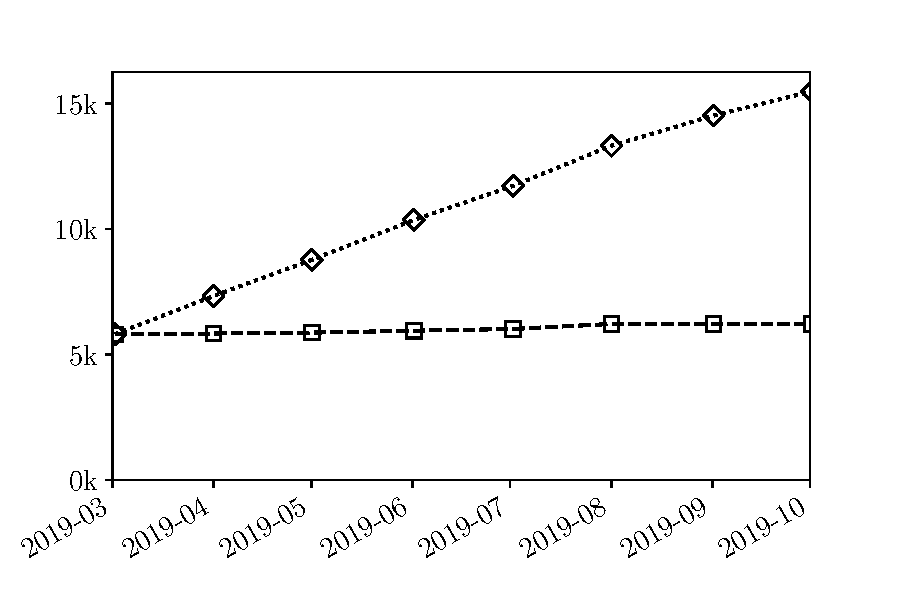
\includegraphics[width=0.5\textwidth]{figures/fig3d.pdf}} \\
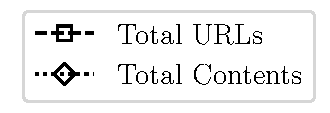
\includegraphics[scale=0.6]{figures/fig3legend.pdf}%

\caption[Network URL and content counts over time]{Total number of URLs and unique contents observed from March 2019 through May 2020 in the provider networks of \subref{fig:network-growth-a} BHL, \subref{fig:network-growth-b} DataONE, \subref{fig:network-growth-c} GBIF, and \subref{fig:network-growth-d} iDigBio.
}%

\label{fig:network-growth} % \label works only AFTER \caption within figure environment

\end{figure}


\begin{figure}[!p] %s state preferences regarding figure placement here

% use to correct figure counter if necessary
%\renewcommand{\thefigure}{2}

\centering
\subfigure[URL reference]{%
\label{fig:verification-a}%
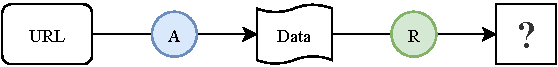
\includegraphics[scale=0.74, right]{figures/fig4a.pdf}} \\
\subfigure[URL reference with content hash]{%
\label{fig:verification-b}%
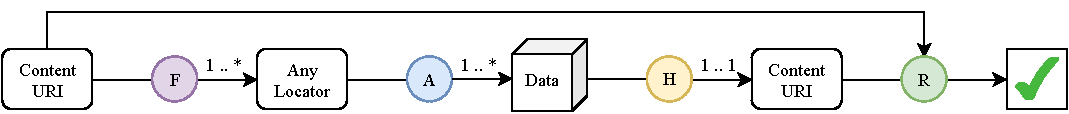
\includegraphics[scale=0.74, right]{figures/fig4b.pdf}} \\
\subfigure[Content URI reference]{%
\label{fig:verification-c}%
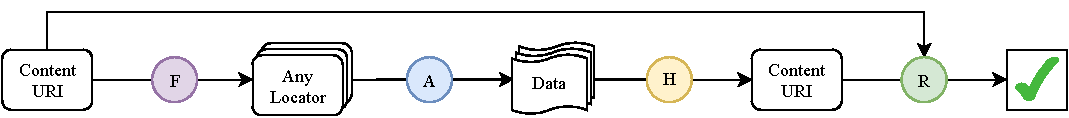
\includegraphics[scale=0.74, right]{figures/fig4c.pdf}} \\
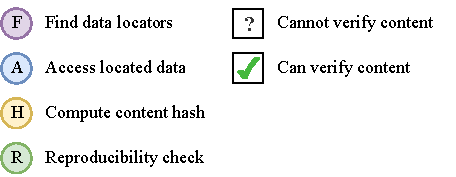
\includegraphics[scale=.9]{figures/fig4legend.pdf}%

\caption{Content resolution and verification for references that use location- versus content-based identifiers. \subref{fig:verification-a} Location-based identifiers (e.g. URLs) cannot verify the authenticity of retrieved content and are vulnerable to link rot due to the use of a fixed locator. \subref{fig:verification-b} If the content hash of the referenced data is known, the authenticity of retrieved data can be verified by comparing the hash of the retrieved data with the provided content hash. However, the fixed locator is still vulnerable to link rot. \subref{fig:verification-c} Content-based identifiers (e.g. Content URIs) can be used to find several locators for the referenced data and contain a content hash to verify the authenticity of retrieved data. The decoupling of the reference from a fixed locator makes the reference resistant to link rot.
}%

\label{fig:verification} % \label works only AFTER \caption within figure environment

\end{figure}

\begin{figure}[t] %s state preferences regarding figure placement here

% use to correct figure counter if necessary
%\renewcommand{\thefigure}{2}

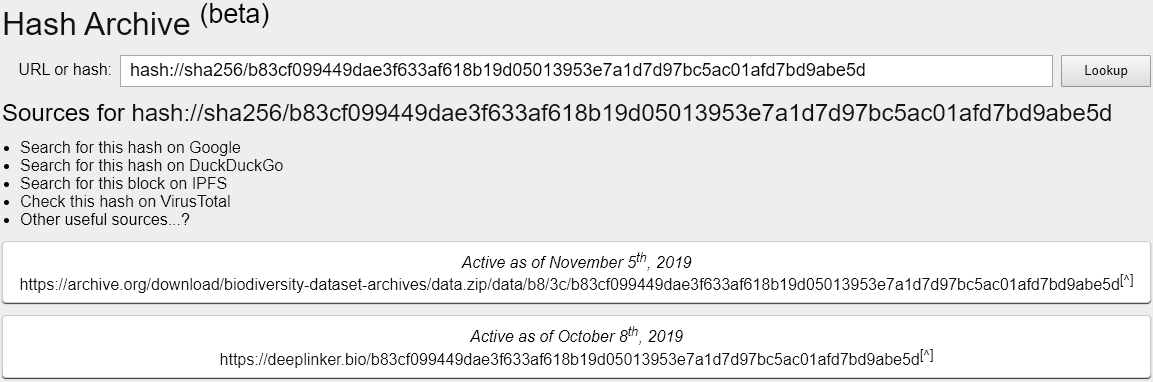
\includegraphics[width=\textwidth]{figures/fig5_grayscale.png}

\caption{An example of a search index mapping hashes to archives. A search for a content or provenance hash at hash-archive.org will find any associated URLs that have been registered at hash-archive.org.}

\label{fig5} % \label works only AFTER \caption within figure environment

\end{figure}


%--------------------------------------------------------%
%	TABLES
%--------------------------------------------------------%

% NOTE: If your submission guidelines don't require tables
% at the end, you can comment out the two lines below,
% and embed tables in the text of content.tex instead of here

\clearpage
\newpage
\section*{Tables}

\begin{table}[!ht]
\begin{adjustwidth}{0in}{0in} % comment out/remove adjustwidth environment if table fits in text column.
\centering
\begin{tabular}{llll}
\hline
{\bf Data Network} & {\bf Responsive URLs} & {\bf Stable URLs*} & {\bf Reliable URLs} \\ \hline
BHL\textsuperscript{a} & 57.41\% (142,672) & 99.97\% (232,996) & 57.39\% (142,633) \\
DataONE\textsuperscript{b} & 94.55\% (352,438) & 92.27\% (339,109) & 87.09\% (324,641) \\
GBIF\textsuperscript{c} & 71.72\% (49,707) & 37.35\% (20,094) & 24.05\% (16,669) \\
iDigBio\textsuperscript{c} & 88.04\% (5,477) & 68.69\% (4,251) & 61.68\% (3,837)  \\
All observed URLs** & 78.94\% (546,645) & 90.43\% (593,469) & 70.07\% (485,203) \\ \hline
\end{tabular}
\caption{Overall responsiveness, stability, and reliability for URLs observed in each biodiversity data network and for all observed URLs as of October 2019.
*URLs that never provided content were omitted from the divisor when calculating Stable URLs percentages.
**Because URLs may be registered in more than one data network, the total number of observed URLs is expected to be less than the sum of the URL counts for each network.
\textsuperscript{a}\citet{poelen_jorrit_h_2019_3484555}
\textsuperscript{b}\citet{poelen_jorrit_h_2019_3483218}
\textsuperscript{c}\citet{poelen_jorrit_h_2019_3484205}
}
\label{table1}
\end{adjustwidth}
\end{table}


\end{document}
